% Asset ID: A21AlgebraicMethodsProofByContradictionTikZ-002
% Source: Dr Frost negation slide; teacher transcript; Phase 1 Key Definitions and Notation
% Related lesson section: Key Definitions and Notation
% Purpose: Show correct negations for common statement forms.
\documentclass[tikz,border=8pt]{standalone}
\usepackage{amsmath}
\usetikzlibrary{arrows.meta,positioning}
\begin{document}
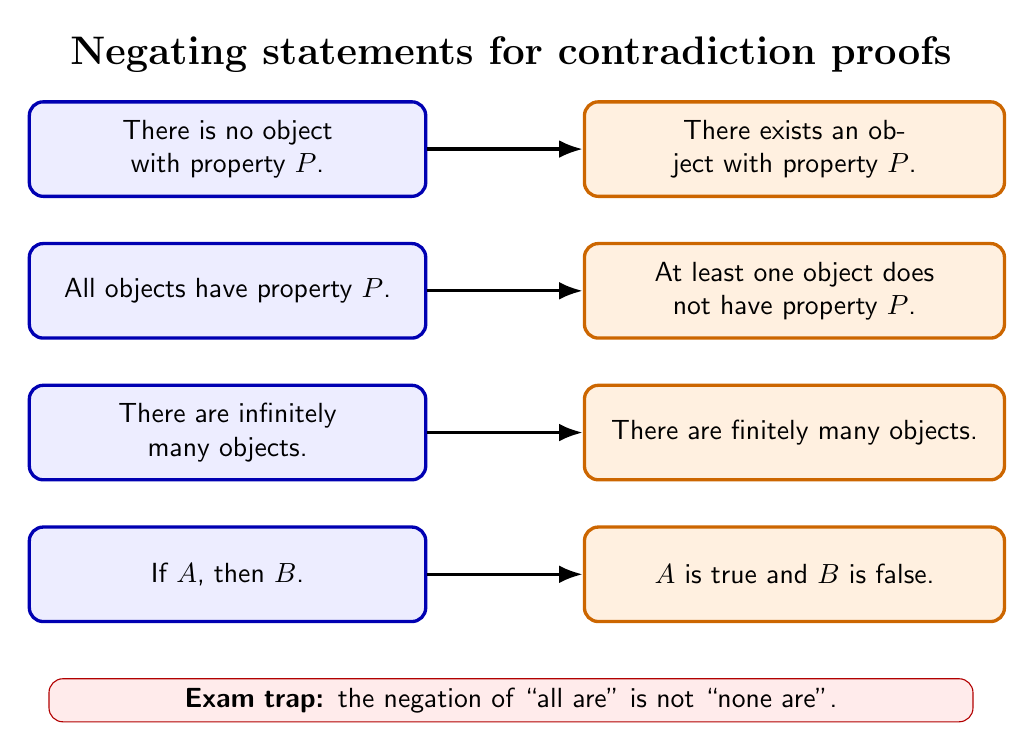
\begin{tikzpicture}[font=\sffamily, original/.style={rectangle, rounded corners=5pt, draw=blue!70!black, very thick, fill=blue!7, text width=4.8cm, align=center, minimum height=1.2cm}, negation/.style={rectangle, rounded corners=5pt, draw=orange!80!black, very thick, fill=orange!12, text width=5.1cm, align=center, minimum height=1.2cm}, arrow/.style={-{Latex[length=3mm]}, very thick}]
\node[font=\bfseries\Large] at (3.6,1.2) {Negating statements for contradiction proofs};
\node[original] (o1) at (0,0) {There is no object with property $P$.};
\node[negation] (n1) at (7.2,0) {There exists an object with property $P$.};
\node[original] (o2) at (0,-1.8) {All objects have property $P$.};
\node[negation] (n2) at (7.2,-1.8) {At least one object does not have property $P$.};
\node[original] (o3) at (0,-3.6) {There are infinitely many objects.};
\node[negation] (n3) at (7.2,-3.6) {There are finitely many objects.};
\node[original] (o4) at (0,-5.4) {If $A$, then $B$.};
\node[negation] (n4) at (7.2,-5.4) {$A$ is true and $B$ is false.};
\draw[arrow] (o1) -- (n1); \draw[arrow] (o2) -- (n2); \draw[arrow] (o3) -- (n3); \draw[arrow] (o4) -- (n4);
\node[rectangle, rounded corners=5pt, draw=red!70!black, fill=red!8, align=center, text width=11.5cm] at (3.6,-7.0) {\textbf{Exam trap:} the negation of ``all are'' is not ``none are''.};
\end{tikzpicture}
\end{document}
